\begin{frame}{A smoother fin handover improves RMS and moves the minimum earlier}
\begin{columns}[c,onlytextwidth]
\column{.65\linewidth}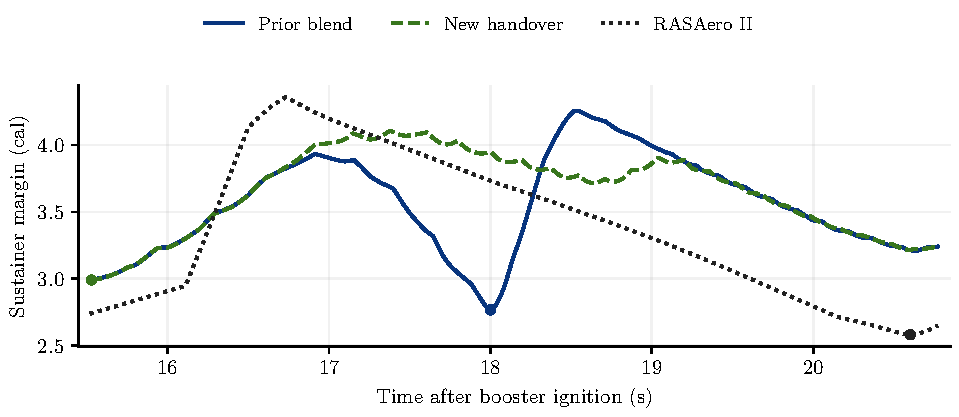
\includegraphics[width=\linewidth]{figures/handover-flight.pdf}
\column{.32\linewidth}\small
Burn-wide margin RMS falls from 0.56 to 0.44 cal.\\[.7em]
The new minimum occurs at 15.53 s. RASAero reaches its minimum at 20.60 s.\\[.7em]
Burnout remains about 3.24 cal, compared with 2.65 in RASAero.
\end{columns}
\begin{block}{Iris component test at Mach 2.80 and 2 degrees}
\small The aft airframe accounts for $+0.33\,D$ of CP error, installed fins for $+0.13\,D$, and the bare forebody for $-0.15\,D$. Removing the camera drag area leaves native CP and normal force unchanged on 906 tested states.
\end{block}
\end{frame}
\begin{frame}{Measured wing--body interference exposes a remaining model error}
\begin{columns}[c,onlytextwidth]
\column{.61\linewidth}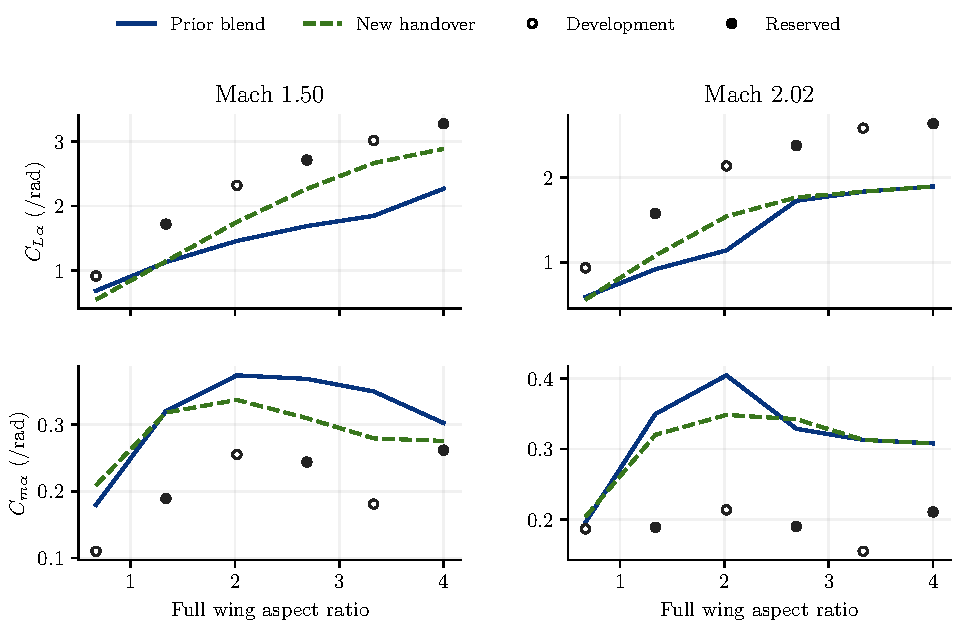
\includegraphics[width=\linewidth]{figures/handover-tn3795.pdf}
\column{.36\linewidth}\small
\textbf{NACA TN 3795}\\Three reserved wings at two Mach numbers. Assembled lift-slope RMS falls from 0.80 to 0.55/rad.\\[.6em]
The isolated interaction worsens. Measured mean lift interference is $-0.26$/rad versus $-0.79$/rad in the new model.\\[.6em]
Keep the prior research blend. The handover experiment identifies the crossover behavior and the aft-airframe load discrepancy.
\end{columns}
\end{frame}
